% Options for packages loaded elsewhere
\PassOptionsToPackage{unicode}{hyperref}
\PassOptionsToPackage{hyphens}{url}
%
\documentclass[
  man]{apa6}
\usepackage{amsmath,amssymb}
\usepackage{iftex}
\ifPDFTeX
  \usepackage[T1]{fontenc}
  \usepackage[utf8]{inputenc}
  \usepackage{textcomp} % provide euro and other symbols
\else % if luatex or xetex
  \usepackage{unicode-math} % this also loads fontspec
  \defaultfontfeatures{Scale=MatchLowercase}
  \defaultfontfeatures[\rmfamily]{Ligatures=TeX,Scale=1}
\fi
\usepackage{lmodern}
\ifPDFTeX\else
  % xetex/luatex font selection
\fi
% Use upquote if available, for straight quotes in verbatim environments
\IfFileExists{upquote.sty}{\usepackage{upquote}}{}
\IfFileExists{microtype.sty}{% use microtype if available
  \usepackage[]{microtype}
  \UseMicrotypeSet[protrusion]{basicmath} % disable protrusion for tt fonts
}{}
\makeatletter
\@ifundefined{KOMAClassName}{% if non-KOMA class
  \IfFileExists{parskip.sty}{%
    \usepackage{parskip}
  }{% else
    \setlength{\parindent}{0pt}
    \setlength{\parskip}{6pt plus 2pt minus 1pt}}
}{% if KOMA class
  \KOMAoptions{parskip=half}}
\makeatother
\usepackage{xcolor}
\usepackage{graphicx}
\makeatletter
\def\maxwidth{\ifdim\Gin@nat@width>\linewidth\linewidth\else\Gin@nat@width\fi}
\def\maxheight{\ifdim\Gin@nat@height>\textheight\textheight\else\Gin@nat@height\fi}
\makeatother
% Scale images if necessary, so that they will not overflow the page
% margins by default, and it is still possible to overwrite the defaults
% using explicit options in \includegraphics[width, height, ...]{}
\setkeys{Gin}{width=\maxwidth,height=\maxheight,keepaspectratio}
% Set default figure placement to htbp
\makeatletter
\def\fps@figure{htbp}
\makeatother
\setlength{\emergencystretch}{3em} % prevent overfull lines
\providecommand{\tightlist}{%
  \setlength{\itemsep}{0pt}\setlength{\parskip}{0pt}}
\setcounter{secnumdepth}{-\maxdimen} % remove section numbering
% Make \paragraph and \subparagraph free-standing
\makeatletter
\ifx\paragraph\undefined\else
  \let\oldparagraph\paragraph
  \renewcommand{\paragraph}{
    \@ifstar
      \xxxParagraphStar
      \xxxParagraphNoStar
  }
  \newcommand{\xxxParagraphStar}[1]{\oldparagraph*{#1}\mbox{}}
  \newcommand{\xxxParagraphNoStar}[1]{\oldparagraph{#1}\mbox{}}
\fi
\ifx\subparagraph\undefined\else
  \let\oldsubparagraph\subparagraph
  \renewcommand{\subparagraph}{
    \@ifstar
      \xxxSubParagraphStar
      \xxxSubParagraphNoStar
  }
  \newcommand{\xxxSubParagraphStar}[1]{\oldsubparagraph*{#1}\mbox{}}
  \newcommand{\xxxSubParagraphNoStar}[1]{\oldsubparagraph{#1}\mbox{}}
\fi
\makeatother
% definitions for citeproc citations
\NewDocumentCommand\citeproctext{}{}
\NewDocumentCommand\citeproc{mm}{%
  \begingroup\def\citeproctext{#2}\cite{#1}\endgroup}
\makeatletter
 % allow citations to break across lines
 \let\@cite@ofmt\@firstofone
 % avoid brackets around text for \cite:
 \def\@biblabel#1{}
 \def\@cite#1#2{{#1\if@tempswa , #2\fi}}
\makeatother
\newlength{\cslhangindent}
\setlength{\cslhangindent}{1.5em}
\newlength{\csllabelwidth}
\setlength{\csllabelwidth}{3em}
\newenvironment{CSLReferences}[2] % #1 hanging-indent, #2 entry-spacing
 {\begin{list}{}{%
  \setlength{\itemindent}{0pt}
  \setlength{\leftmargin}{0pt}
  \setlength{\parsep}{0pt}
  % turn on hanging indent if param 1 is 1
  \ifodd #1
   \setlength{\leftmargin}{\cslhangindent}
   \setlength{\itemindent}{-1\cslhangindent}
  \fi
  % set entry spacing
  \setlength{\itemsep}{#2\baselineskip}}}
 {\end{list}}
\usepackage{calc}
\newcommand{\CSLBlock}[1]{\hfill\break\parbox[t]{\linewidth}{\strut\ignorespaces#1\strut}}
\newcommand{\CSLLeftMargin}[1]{\parbox[t]{\csllabelwidth}{\strut#1\strut}}
\newcommand{\CSLRightInline}[1]{\parbox[t]{\linewidth - \csllabelwidth}{\strut#1\strut}}
\newcommand{\CSLIndent}[1]{\hspace{\cslhangindent}#1}
\ifLuaTeX
\usepackage[bidi=basic]{babel}
\else
\usepackage[bidi=default]{babel}
\fi
\babelprovide[main,import]{english}
% get rid of language-specific shorthands (see #6817):
\let\LanguageShortHands\languageshorthands
\def\languageshorthands#1{}
% Manuscript styling
\usepackage{upgreek}
\captionsetup{font=singlespacing,justification=justified}

% Table formatting
\usepackage{longtable}
\usepackage{lscape}
% \usepackage[counterclockwise]{rotating}   % Landscape page setup for large tables
\usepackage{multirow}		% Table styling
\usepackage{tabularx}		% Control Column width
\usepackage[flushleft]{threeparttable}	% Allows for three part tables with a specified notes section
\usepackage{threeparttablex}            % Lets threeparttable work with longtable

% Create new environments so endfloat can handle them
% \newenvironment{ltable}
%   {\begin{landscape}\centering\begin{threeparttable}}
%   {\end{threeparttable}\end{landscape}}
\newenvironment{lltable}{\begin{landscape}\centering\begin{ThreePartTable}}{\end{ThreePartTable}\end{landscape}}

% Enables adjusting longtable caption width to table width
% Solution found at http://golatex.de/longtable-mit-caption-so-breit-wie-die-tabelle-t15767.html
\makeatletter
\newcommand\LastLTentrywidth{1em}
\newlength\longtablewidth
\setlength{\longtablewidth}{1in}
\newcommand{\getlongtablewidth}{\begingroup \ifcsname LT@\roman{LT@tables}\endcsname \global\longtablewidth=0pt \renewcommand{\LT@entry}[2]{\global\advance\longtablewidth by ##2\relax\gdef\LastLTentrywidth{##2}}\@nameuse{LT@\roman{LT@tables}} \fi \endgroup}

% \setlength{\parindent}{0.5in}
% \setlength{\parskip}{0pt plus 0pt minus 0pt}

% Overwrite redefinition of paragraph and subparagraph by the default LaTeX template
% See https://github.com/crsh/papaja/issues/292
\makeatletter
\renewcommand{\paragraph}{\@startsection{paragraph}{4}{\parindent}%
  {0\baselineskip \@plus 0.2ex \@minus 0.2ex}%
  {-1em}%
  {\normalfont\normalsize\bfseries\itshape\typesectitle}}

\renewcommand{\subparagraph}[1]{\@startsection{subparagraph}{5}{1em}%
  {0\baselineskip \@plus 0.2ex \@minus 0.2ex}%
  {-\z@\relax}%
  {\normalfont\normalsize\itshape\hspace{\parindent}{#1}\textit{\addperi}}{\relax}}
\makeatother

\makeatletter
\usepackage{etoolbox}
\patchcmd{\maketitle}
  {\section{\normalfont\normalsize\abstractname}}
  {\section*{\normalfont\normalsize\abstractname}}
  {}{\typeout{Failed to patch abstract.}}
\patchcmd{\maketitle}
  {\section{\protect\normalfont{\@title}}}
  {\section*{\protect\normalfont{\@title}}}
  {}{\typeout{Failed to patch title.}}
\makeatother

\usepackage{xpatch}
\makeatletter
\xapptocmd\appendix
  {\xapptocmd\section
    {\addcontentsline{toc}{section}{\appendixname\ifoneappendix\else~\theappendix\fi\\: #1}}
    {}{\InnerPatchFailed}%
  }
{}{\PatchFailed}
\keywords{Reproducibility, R, Self-bias, Positive-bias, Self-positive-bias}
\DeclareDelayedFloatFlavor{ThreePartTable}{table}
\DeclareDelayedFloatFlavor{lltable}{table}
\DeclareDelayedFloatFlavor*{longtable}{table}
\makeatletter
\renewcommand{\efloat@iwrite}[1]{\immediate\expandafter\protected@write\csname efloat@post#1\endcsname{}}
\makeatother
\usepackage{lineno}

\linenumbers
\usepackage{csquotes}
\ifLuaTeX
  \usepackage{selnolig}  % disable illegal ligatures
\fi
\usepackage{bookmark}
\IfFileExists{xurl.sty}{\usepackage{xurl}}{} % add URL line breaks if available
\urlstyle{same}
\hypersetup{
  pdftitle={Verification of computational reproducibility for the research results of Lee et al.(2023).},
  pdfauthor={Jiaqi Wu1, Kangmiao Wei1, Qian Li1, \& Jiajie Wang1},
  pdflang={en-EN},
  pdfkeywords={Reproducibility, R, Self-bias, Positive-bias, Self-positive-bias},
  hidelinks,
  pdfcreator={LaTeX via pandoc}}

\title{Verification of computational reproducibility for the research results of Lee et al.(2023).}
\author{Jiaqi Wu\textsuperscript{1}, Kangmiao Wei\textsuperscript{1}, Qian Li\textsuperscript{1}, \& Jiajie Wang\textsuperscript{1}}
\date{}


\shorttitle{papaja}

\authornote{

The authors made the following contributions. Jiaqi Wu: Writing - Methods \& Abstract, Writing - Integrate and revise the text; Kangmiao Wei: Writing - Discussion; Qian Li: Writing - Introduction; Jiajie Wang: Writing - Results.

Correspondence concerning this article should be addressed to Jiaqi Wu, \#122 Ninghai Rd, Gulou District, Nanjing. E-mail: \href{mailto:wujiaqipsy@foxmail.com}{\nolinkurl{wujiaqipsy@foxmail.com}}

}

\affiliation{\vspace{0.5cm}\textsuperscript{1} Nanjing Normal Unviersity}

\abstract{%
While the effects of self-bias and positivity-bias have been well documented in isolation, their examination in parallel has been limited, leaving uncertainty about their prioritization and potential interaction. To address this gap, Lee et al.~(2023) designed a classification task that paired self-relevant information with emotional expressions, aiming to determine the relative primacy of self-bias and positivity-bias. We replicated Experiment 1 from Lee et al.'s 2023 study and found minor discrepancies in our results compared to the original findings. However, our replication supported the same conclusions. When the self was associated with more positive information, such as smiling faces, we observed evidence of self-bias but not positivity-bias. Conversely, when the self was paired with less positive information, like neutral faces, we detected evidence of positivity-bias but not self-bias. These findings suggest that the processing priority is flexible and context-dependent, potentially driven by a motivation for self-enhancement and a self-positivity bias.
}



\begin{document}
\maketitle

\section{1 Introduction}\label{introduction}

\subsection{1.1 Division of labor among team members}\label{division-of-labor-among-team-members}

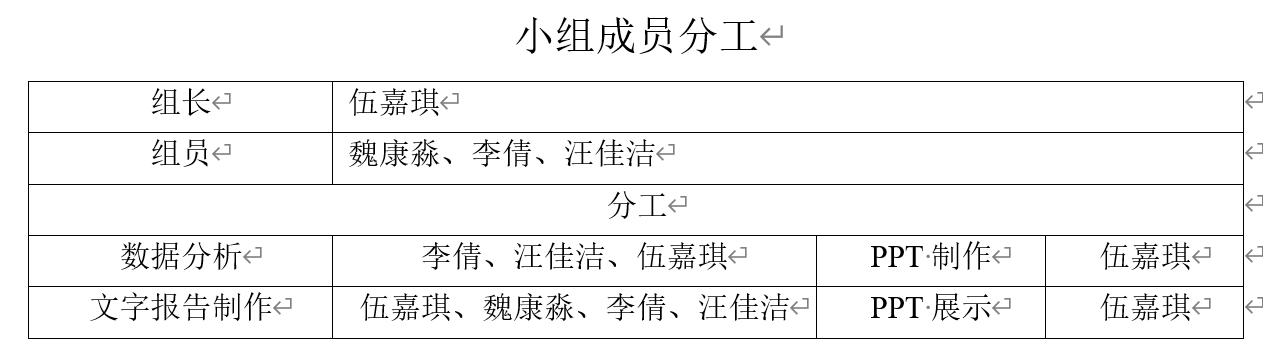
\includegraphics{pic/FenGong.png}

\subsection{1.2 Selected Literature}\label{selected-literature}

\textbf{Citation:}Lee, N. A., Martin, D., \& Sui, J. (2023). Accentuate the positive: Evidence that context dependent self-reference drives self-bias. Cognition, 240, 105600.

\textbf{Data and Code:}\url{https://osf.io/4k56b/?view_only=6575952710034f5b867f83aebdca9112}

\subsection{1.2 Literature Review}\label{literature-review}

The aim of the current research was to examine the relative primacy between self-biases and positivity-biases -- does one form of bias exert a greater influence than the other? To successfully navigate the complex human environment people must selectively orient their spotlight of attention and appropriately allocate their limited cognitive resources. This means prioritising some aspects of the environment more than others. There are multiple convincing demonstrations of a self-bias whereby people show prioritised processing towards self-related stimuli such as own names (Moray, 1959), faces (Sui \& Humphreys, 2013; Tong \& Nakayama, 1999) and objects (Golubickis et al., 2021; Turk et al., 2011). There is also abundant evidence of a positivity-bias whereby people show prioritised processing towards positively valenced stimuli such as smiling faces (Hugdahl, Iversen, \& Johnsen, 1993), positive words (Stenberg, Wiking, \& Dahl, 1998), and high rewards (Anderson, Laurent, \& Yantis, 2011).

To date, research has focused unidirectionally on the influence of pairing positive and negative stimuli with the self. Therefore, it remains unknown whether the self-positivity-bias will also influence positivity-biases. Across two experiments, the current research sought to address the previously presented questions to establish the relative primacy between self-biases and positivity-biases by adapting a speeded classification task (Sui \& Humphreys, 2015).

The current research employed a classification task where Experiment 1 explored the relationship between the self and positive/neutral facial expressions. Experiment 2 examined the relationship between the self and high/low rewards; the procedure was identical to Experiment 1 except that the labels of happy and neutral were replaced with high reward and low reward (£9 and £1 respectively), to determine the relative primacy between self-biases and positivity-biases.

Thus, the current research aimed to determine:

1. Self-bias occurs irrespective of the relative positivity of stimulus pairings (i.e., context independent self-bias)

2. Positivity-bias occurs irrespective of the relative self-relevance of stimulus pairings (i.e., context independent positivity bias)

3. Self-bias will be larger, or uniquely present, when the self is paired with more positive stimuli (i.e., context dependent self-enhancing bias)

The results of the two experiments indicated that self-biases and positivity-biases change under different conditions and that these biases are influenced by the pairing between self and positive stimuli. Specifically, self-biases were observed when the self was paired with positivity but were eliminated when the self was paired with neutrality. Conversely, positivity-biases were observed when positivity was paired with friends but not when paired with the self. These findings provide new experimental support for the relative primacy of self-biases and positivity-biases in cognition. Humans have a remarkable ability to store large numbers of images in visual long-term memory(VLTM), but not all visual information can be remembered equally well.

\section{2 Methods}\label{methods}

\subsection{2.1 The original research methodology}\label{the-original-research-methodology}

Using R version 4.4.0, we replicated the results of Experiment 1. The data used was the processed data which contains data from 47 participants, yet the experiment collected 57 participants' data. The code for analysis was provided by the original article, which has been annotated for clarification.

Experiment design:Experiment 1 was a within-subjects 4 (Individual association: Self, Friend, Happy, Neutral) X 2 (Condition: 1-Self \& Happy/Friend \& Neutral pairings vs.~2-Self \& Neutral/Friend \& Happy pairings) design.

Experiment Procedure: In experiment 1, participants need to finish two tasks: shape-label matching task and classification task. During an initial shape-label matching (Sui, He, \& Humphreys, 2012) training phase, participants learnt associations between four geometric shapes and four labels. They were told that shapes would represent themselves, a previously named best friend, a happy face and neutral face and were tested on these associations. Sui et al.~(2012) matching task was used to train the associations of shapes and labels. During the classification task, participants were instructed that shapes would be paired together onto a single response key and that when a shape appeared they should press the corresponding key as quickly and accurately as possible. In Condition 1, the pairs were: Self and Happy, Friend and Neutral. In Condition 2, the pairs were: Self and Neutral, Friend and Happy. In a single trial, following fixation, shapes were presented (singularly left or right of the fixation cross, or two shapes both left and right). Subsequently participants made a speeded judgment as to which pairing the shape/s belong to. Feedback (correct, incorrect, too slow) followed each trial. Average reaction time (RT) and accuracy were reported at the end of each block. There were three practice blocks. For the experimental task, participants completed three blocks of 60 trials resulting in 30 trials in each factor equally presented to the left and right (i.e., Individual association: self, friend, happy, neutral; and Paired: self and happy/neutral, friend and happy/neutral). The current work focused on individual association trial types, the paired trials were present to ensure pairings were retained, but are not analysed in this manuscript. Between conditions participants completed questionnaires which will be used in future research and are not reported here.

\subsection{2.2 Replication approach and R packages}\label{replication-approach-and-r-packages}

Researcher proposed three hypotheses. First, Self-bias occurs irrespective of the relative positivity of stimulus pairings (i.e., context independent self-bias). Second, Positivity-bias occurs irrespective of the relative self-relevance of stimulus pairings (i.e., context independent positivity bias). Third, Self-bias will be larger, or uniquely present, when the self is paired with more positive stimuli (i.e., context dependent self-enhancing bias).To test the above hypothesizes, researchers used GLMMs to test two-way interactions between fixed effects: individual association (self, friend, happy, neutral), and condition(Condition 1: Self/Happy, Friend/Neutral pairings vs.~Condition 2: Self/Neutral, Friend/Happy pairings) and set the dependent variable as response time or accuracy.

The data analysis process, leveraging a range of R packages, is structured into three key components: data preprocessing, descriptive statistics, and inferential statistics. Data cleaning, transformation, and manipulation are handled by dplyr and tidyr, with additional support from languageR. For inferential statistics, lme4 is used to fit GLMMs, with emmeans for post-hoc comparisons. Visualization and presentation of model results are facilitated by sjPlot and ggplot2, while forcats aids in ordering factor levels. The GLMMs' validity is assessed using DHARMa, and stringr is used for string manipulation. Predictive plots are generated with ggeffects, and results are formatted in APA style using papaja. For plot combination, cowplot, ggpubr, and patchwork are used, ensuring a cohesive workflow from data preparation to the final presentation of findings.

To begin with data preprocessing, the dataset is loaded, and the variables within it are renamed to enhance clarity. This step includes renaming the levels of the \texttt{Association} variable and standardizing the names of the \texttt{trial\_type} and \texttt{Condition} variables. The data is then cleaned by removing trials with extremely short reaction times (RTs) less than 200ms, and the dataset is filtered to isolate categorical task data. The proportion of trials with RTs below 200ms and those exceeding 1650ms (indicating a timeout) are calculated. Subsequently, single-stimulus trials are extracted for further analysis.

In the descriptive statistics phase, the analysis focuses on providing a summary of the data. This includes determining the number of male and female participants and calculating descriptive measures such as the mean, standard deviation, maximum, and minimum for the age variable.

The inferential statistics component involves a more in-depth examination of the data to draw conclusions about the population. This is done by converting the data into factors, applying non-orthogonal coding, and selecting only the correct trials for analysis. Generalized linear mixed models (GLMMs) are then used to analyze both reaction times and accuracy rates. This entails fitting GLMMs to the RT data, presenting the fitting results, conducting simple effects analysis for interactions, and visualizing the outcomes. A parallel process is followed for the accuracy rates, including fitting GLMMs, presenting the results, and visualizing the interactions.

\section{3 Results}\label{results}

For the data of experiment 1, the results we reproduced by using the original code were roughly the same as those in the original literature. The three hypotheses have been verified, no matter under which conditions, there will be self bias and positive bias. and the two are not mutually exclusive, and in the situation of self and positive pairing, the effect of self bias will increase.

\subsection{3.1 Descriptive statistics}\label{descriptive-statistics}

The author first preprocessed the data. The data whose RT was less than 200ms were mainly eliminated. The attempts of RT \textless{} 200ms and RT \textgreater{} 1650ms in the classification task were calculated respectively. The author did not eliminate the data whose rejection response timeout appeared ceiling effect after deletion, and we also found the same result when deleting data. The author calculated the total number of attempts to be 16920, and we obtained the total number of attempts to be 16766 after subtracting the number of attempts less than 200ms.

Then descriptive statistical analysis was carried out to calculate The number and age distribution of male and female students. the author's result was as follows: The average age of the 47 participants was 20.23 years (\emph{SD} = 1.92, range = 18-28). There are some differences in the age distribution of our calculations (\emph{M} = 20.24, \emph{SD} = 1.92, range = 18-28). The author's results can be replicated. The replication of descriptive statistics is presented in Table 1.

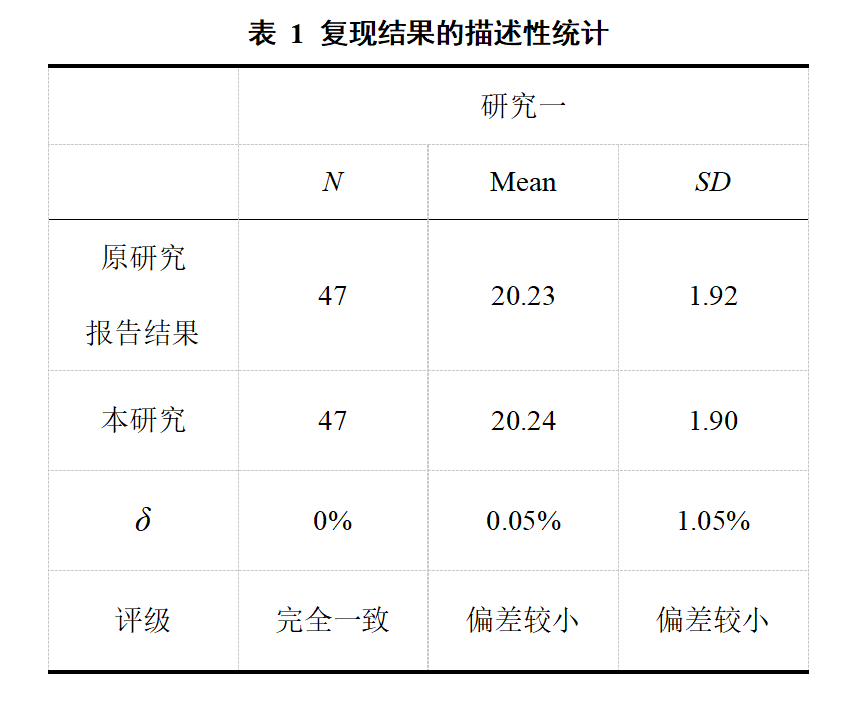
\includegraphics{pic/table1.png}

\subsection{3.2 Inferential statistics}\label{inferential-statistics}

The authors then use the generalized linear mixed effects model of lme4 package to verify the fixed and interactive effects, and calculate the model fit and random effects. In order to verify H1 and H2, that is, whether self-bias and positive bias exist under different circumstances, the author first converted the columns Condition and Association into factor variables, customized factor levels, and used the levels function to check, and created data sets of RT and ACC. Generalized linear mixing model glmer when running reaction in formal steps: RT \textasciitilde{} person * prime * condition + (1\textbar participant), fitted GLMM and performed summary statistics on the fitting results. The random effects of age were added to re-run the model. Finally, a brief overview of fixed effects and random effects in the model was presented. It includes model coefficient, standard error, z value and p value. The result of the original text is: H1. A significant two-way interaction indicated differences across the conditions between self-bias magnitudes (\(\beta\) = -47.58, 95\% CI {[}-60.84,-34.32{]}, \emph{p} \textless{} .001); H2. Like self-bias, a significant two-way interaction indicated changes in emotional positivity-bias magnitudes across conditions (\(\beta\) = 28.47, 95\% CI {[}14.31,42.62{]}, \emph{p} \textless{} .001).The result we reproduced was: H1. \(\beta\) = - 47.58, 95\% CI {[}-60.85,-34.31{]}, \emph{p} \textless{} .001; H2.\(\beta\) = 28.47, 95\% CI {[}14.63,42.30{]}, \emph{p} \textless{} .001, which are roughly the same as the author's results.

In cases where the interaction between Condition and Individual association is significant, the emmeans package is used for post hoc analysis. To test H3, that is, whether the self-bias effect increases in situations where the self is paired with positivity. The authors first create vectors for each set of average values of a particular ppair comparison, and then examine the differences in reaction time between self and friend under different conditions and between different conditions, the differences in reaction time under different emotional conditions, and the interaction between different conditions and the interaction effect between self and emotional conditions, and the interaction between different conditions. The result of the original text is: H3. Posthoc analysis revealed a significant self-bias in individual associations in Condition 1 when the self was paired with the happy face (friend with neutral) (\(\beta\) = -24.79, 95\% CI {[}-33.91,-15.67{]}, \emph{p} \textless{} .0001).The result we reproduced was: H3.\(\beta\) = - 24.79, 95\% CI {[}-33.85,-15.73{]}, \emph{p} \textless{} .0001. The results we reproduced using the original code are roughly the same as the author's results. The replication of descriptive statistics is presented in Table 2.

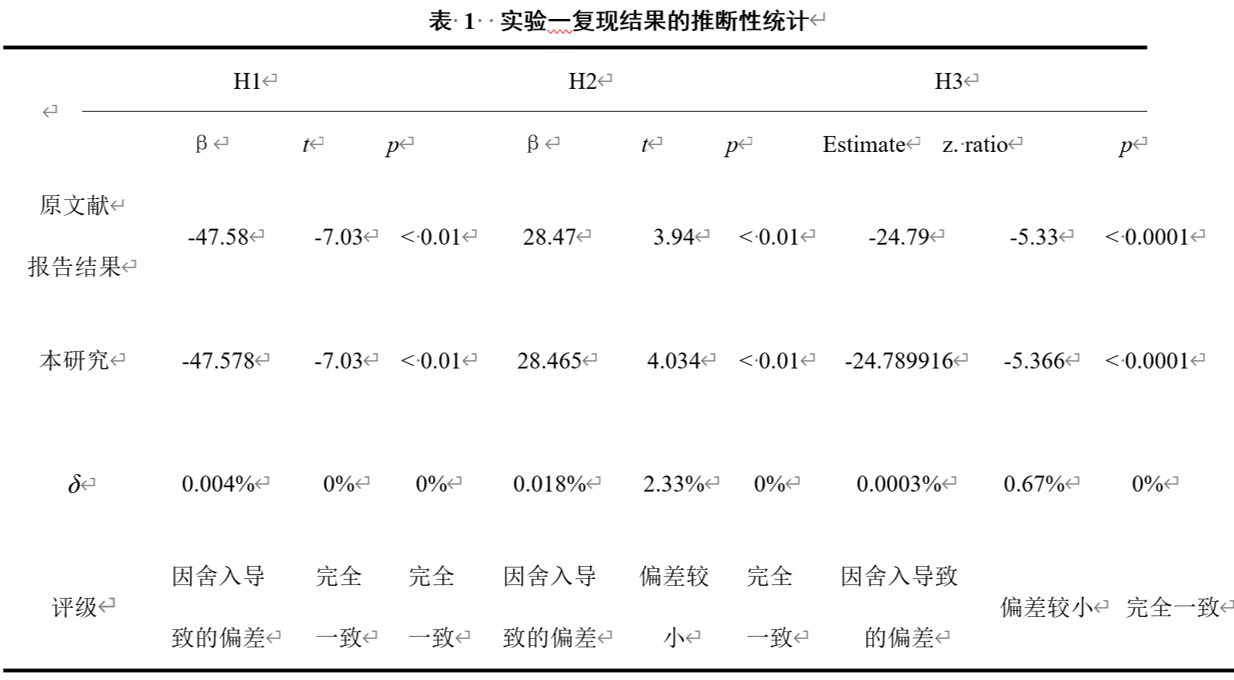
\includegraphics{pic/table2.png}

\subsection{3.3 Summary of Computational Replicability Results}\label{summary-of-computational-replicability-results}

In this study, we successfully replicated all the key statistical results of the original literature. By implementing precise R code, we conducted a comprehensive examination of both the descriptive and inferential statistics reported in the original literature. The results of our analysis are in complete agreement with the results reported in the original literature, demonstrating the high reproducibility of the original study.The computational reproducibility of the study is presented in Table 3.

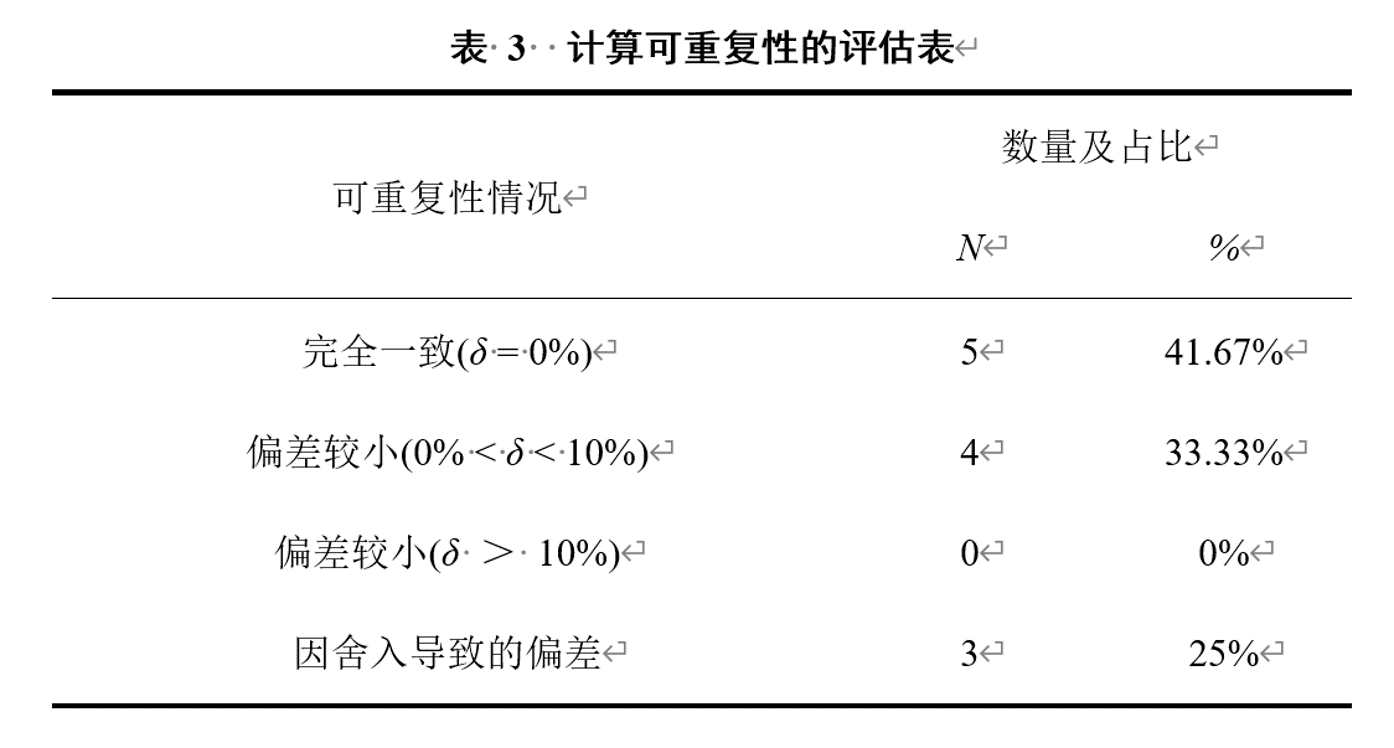
\includegraphics{pic/table3.png}

\section{4 Discussion}\label{discussion}

In this study, we successfully replicated all key statistical results from the original paper. By accurately implementing the R code, we thoroughly examined both the descriptive and inferential statistics reported in the original paper. We found that our analysis results showed some discrepancies compared to those reported in the original paper.

\subsection{4.1 Descriptive Statistics}\label{descriptive-statistics-1}

The original paper reported an average participant age of 20.23 years (\emph{SD} = 1.92, range 18--28), whereas our replication results showed an average age of 20.24 years (\emph{SD} = 1.902, range 18--28). Despite multiple attempts, including removing reaction times below 200 milliseconds(RT\textless200ms) and excluding erroneous trials from participants, the average age and standard deviation still differed from those reported in the original paper.

\subsection{4.2 Inferential Statistics}\label{inferential-statistics-1}

Differences between the original paper and our replication results were observed in the outputs of the generalized linear mixed-effects model and the post-hoc pairwise comparisons. Specifically, the fixed effects' standard errors (\emph{SE}) and t-values(\emph{t}) from the generalized linear model showed discrepancies, and the variance of the random effects also differed. In the post-hoc pairwise comparisons, most standard errors exhibited slight differences, and some p-values(\emph{p}) varied, although these changes did not alter the conclusions regarding statistical significance.

Despite the differences in descriptive and inferential statistics, the \(\beta\)-values(\(\beta\))and p-values in both our replication and the original paper were consistent, indicating that the direction and magnitude of the predictor variables' effects were aligned. This suggests that the main conclusions are reliable, and the other discrepancies did not significantly impact the primary conclusions.

\subsection{4.3 Reasons for Discrepancies}\label{reasons-for-discrepancies}

Analyzing the reasons for inconsistencies between the original literature and the replicated results, there are several possible points to consider:

On one hand, the original article did not provide the complete raw data. It was mentioned that the experiment initially selected 57 participants, with 10 not meeting the test requirements and thus being excluded, but the data from these excluded participants was not provided. There is a slight discrepancy between the sample size reported in the original article and the sample size used in the replication process. Even a difference of a single data point could affect the calculation of the Standard Error.on the other hand, the original article did not provide the original R packages used. Different versions of the R packages might produce subtle computational differences, leading to variations in the data processing results.

Although there are differences in descriptive and inferential statistics, these differences do not impact the reliability of the main conclusions, which remain consistent with the original paper. The findings indicate that self-bias and positivity bias do not manifest consistently across all conditions, failing to support Hypotheses 1 and 2 that self-bias and positivity bias occur regardless of context. Instead, the study found that the relative primacy of self-bias and positivity bias depends on the paired context. Specifically, individuals exhibit self-bias when self-related information is associated with positive factors, prioritizing processing self-related positive information. However, when the self is associated with neutral factors, the bias shifts toward the positive aspects of the external environment.

These findings suggest that to maintain self-positivity, self-referential processing is context-dependent, with self-related stimuli being prioritized only in emotional contexts paired with positive information. This result highlights the critical role of paired contexts in self-bias and positivity bias, providing new perspectives for understanding these biases' mechanisms. Future research should explore whether these biases persist over the long term or change over time and with accumulated experience. Additionally, further investigation is needed to understand how different contexts influence self-referential processing, specifically examining the impact of pairing self with positive information in various emotional backgrounds on self-bias.

\begin{verbatim}
## Generalized linear mixed model fit by maximum likelihood (Laplace
##   Approximation) [glmerMod]
##  Family: inverse.gaussian  ( identity )
## Formula: RT ~ Association * Condition + (1 + Condition | subject)
##    Data: SE_single_RT
## Control: glmerControl(optimizer = "bobyqa", optCtrl = list(maxfun = 2e+05))
## 
##      AIC      BIC   logLik deviance df.resid 
## 122391.8 122478.0 -61183.9 122367.8     9761 
## 
## Scaled residuals: 
##     Min      1Q  Median      3Q     Max 
## -2.4918 -0.6423 -0.1352  0.4465  7.2218 
## 
## Random effects:
##  Groups   Name                Variance  Std.Dev. Corr
##  subject  (Intercept)         9.057e+02 30.09512     
##           ConditionCon vs Inc 1.905e+03 43.64965 0.03
##  Residual                     1.114e-04  0.01055     
## Number of obs: 9773, groups:  subject, 47
## 
## Fixed effects:
##                                        Estimate Std. Error t value Pr(>|z|)    
## (Intercept)                             582.973      8.951  65.130  < 2e-16 ***
## AssociationS vs. F                        2.561      4.126   0.621 0.534718    
## AssociationH vs. N                       13.987      4.101   3.411 0.000648 ***
## AssociationS vs. H                       17.075      4.603   3.709 0.000208 ***
## ConditionCon vs Inc                      -2.513     10.171  -0.247 0.804836    
## AssociationS vs. F:ConditionCon vs Inc  -47.578      7.120  -6.682 2.35e-11 ***
## AssociationH vs. N:ConditionCon vs Inc   28.465      7.297   3.901 9.58e-05 ***
## AssociationS vs. H:ConditionCon vs Inc   40.393      7.765   5.202 1.97e-07 ***
## ---
## Signif. codes:  0 '***' 0.001 '**' 0.01 '*' 0.05 '.' 0.1 ' ' 1
## 
## Correlation of Fixed Effects:
##             (Intr) AsSv.F AsHv.N AsSv.H CndCvI ASvFvI AHvNvI
## AssctnSvs.F  0.001                                          
## AssctnHvs.N -0.004 -0.277                                   
## AssctnSvs.H -0.008 -0.543  0.518                            
## CndtnCnvsIn  0.006  0.026 -0.033 -0.011                     
## AsSv.F:CCvI  0.040 -0.021 -0.046 -0.010  0.045              
## AsHv.N:CCvI -0.046  0.038  0.054  0.005  0.038 -0.204       
## AsSv.H:CCvI -0.059  0.032  0.048 -0.001 -0.003 -0.468  0.435
\end{verbatim}

~

Experiment 1 RT

Predictors

β

std. Error

C.I (95\%)

t

p

Intercept

582.97

8.95

565.43~--~600.52

65.13

\textless0.01

Self vs.~Friend

2.56

4.13

-5.53~--~10.65

0.62

0.53

Happy vs.~Neutral

13.99

4.10

5.95~--~22.03

3.41

\textless0.01

Self vs.~Happy

17.08

4.60

8.05~--~26.10

3.71

\textless0.01

Congruent vs.~Incongruent

-2.51

10.17

-22.45~--~17.42

-0.25

0.80

Self vs.~Friend X Congruent vs.~Incongruent

-47.58

7.12

-61.53~--~-33.62

-6.68

\textless0.01

Happy vs.~Neutral X Congruent vs.~Incongruent

28.46

7.30

14.16~--~42.77

3.90

\textless0.01

Self vs.~Happy X Congruent vs.~Incongruent

40.39

7.76

25.17~--~55.61

5.20

\textless0.01

Random Effects

σ2

0.01

τ00 subject

905.72

τ11 subject.ConditionCon vs Inc

1905.29

ρ01 subject

0.03

ICC

1.00

N subject

47

Observations

9773

Marginal R2 / Conditional R2

0.061 / 1.000

\begin{verbatim}
##  Association Condition        emmean       SE  df asymp.LCL asymp.UCL
##  self        RG_congruent   572.6149 10.61275 Inf  551.8143  593.4155
##  friend      RG_congruent   597.4048 10.58563 Inf  576.6573  618.1522
##  happy       RG_congruent   582.7915 10.64320 Inf  561.9312  603.6518
##  neutral     RG_congruent   584.1067 10.73901 Inf  563.0586  605.1548
##  self        RG_incongruent 573.6943 10.70670 Inf  552.7096  594.6791
##  friend      RG_incongruent 571.1025 10.79181 Inf  549.9509  592.2540
##  happy       RG_incongruent 586.2425 10.67762 Inf  565.3148  607.1703
##  neutral     RG_incongruent 595.8261 10.62053 Inf  575.0102  616.6419
## 
## Confidence level used: 0.95
\end{verbatim}

\begin{verbatim}
##  contrast                                estimate        SE  df z.ratio p.value
##  Congruent Self - Congruent Friend     -24.789891  4.717856 Inf  -5.254  <.0001
##  Incongruent Self - Incongruent Friend   2.591859  4.659051 Inf   0.556  0.5780
##  Congruent Self - Incongruent Self      -1.079443 10.736264 Inf  -0.101  0.9199
##  Congruent Friend - Incongruent Friend  26.302306 10.924327 Inf   2.408  0.0161
\end{verbatim}

\begin{verbatim}
##  contrast                                estimate        SE  df asymp.LCL
##  Congruent Self - Congruent Friend     -24.789891  4.717856 Inf -34.03672
##  Incongruent Self - Incongruent Friend   2.591859  4.659051 Inf  -6.53971
##  Congruent Self - Incongruent Self      -1.079443 10.736264 Inf -22.12213
##  Congruent Friend - Incongruent Friend  26.302306 10.924327 Inf   4.89102
##  asymp.UCL
##  -15.54306
##   11.72343
##   19.96325
##   47.71359
## 
## Confidence level used: 0.95
\end{verbatim}

\begin{verbatim}
##  contrast                                  estimate        SE  df z.ratio
##  Congruent Happy - Congruent Neutral      -1.315206  4.740378 Inf  -0.277
##  Incongruent Happy - Incongruent Neutral  -9.583545  4.901372 Inf  -1.955
##  Congruent Happy - Incongruent Happy      -3.451033 10.792486 Inf  -0.320
##  Congruent Neutral - Incongruent Neutral -11.719372 10.933419 Inf  -1.072
##  p.value
##   0.7814
##   0.0506
##   0.7491
##   0.2838
\end{verbatim}

\begin{verbatim}
##  contrast                                  estimate        SE  df asymp.LCL
##  Congruent Happy - Congruent Neutral      -1.315206  4.740378 Inf -10.60618
##  Incongruent Happy - Incongruent Neutral  -9.583545  4.901372 Inf -19.19006
##  Congruent Happy - Incongruent Happy      -3.451033 10.792486 Inf -24.60392
##  Congruent Neutral - Incongruent Neutral -11.719372 10.933419 Inf -33.14848
##  asymp.UCL
##   7.975764
##   0.022967
##  17.701851
##   9.709735
## 
## Confidence level used: 0.95
\end{verbatim}

\begin{verbatim}
##  contrast                               estimate        SE  df z.ratio p.value
##  Congruent Self - Congruent Happy     -10.176626  4.733419 Inf  -2.150  0.0316
##  Incongruent Self - Incongruent Happy -12.548215  4.682604 Inf  -2.680  0.0074
##  Congruent Self - Incongruent Self     -1.079443 10.736264 Inf  -0.101  0.9199
##  Congruent Happy - Incongruent Happy   -3.451033 10.792486 Inf  -0.320  0.7491
\end{verbatim}

\begin{verbatim}
##  contrast                               estimate        SE  df asymp.LCL
##  Congruent Self - Congruent Happy     -10.176626  4.733419 Inf -19.45396
##  Incongruent Self - Incongruent Happy -12.548215  4.682604 Inf -21.72595
##  Congruent Self - Incongruent Self     -1.079443 10.736264 Inf -22.12214
##  Congruent Happy - Incongruent Happy   -3.451033 10.792486 Inf -24.60392
##  asymp.UCL
##  -0.899296
##  -3.370481
##  19.963248
##  17.701851
## 
## Confidence level used: 0.95
\end{verbatim}

\begin{verbatim}
##  Association   emmean       SE  df asymp.LCL asymp.UCL
##  self        573.1546 9.209509 Inf  555.1043  591.2049
##  friend      584.2536 9.188263 Inf  566.2449  602.2623
##  happy       584.5170 9.193754 Inf  566.4976  602.5364
##  neutral     589.9664 9.174750 Inf  571.9842  607.9486
## 
## Results are averaged over the levels of: Condition 
## Confidence level used: 0.95
\end{verbatim}

\includegraphics{Papaja_Scripts_Re_Lee_2023_group3_2024_files/figure-latex/SE_RT_single: emmeans_test-1.pdf}

\includegraphics{Papaja_Scripts_Re_Lee_2023_group3_2024_files/figure-latex/SE_RTs_RQ2:figure-1.pdf}

\includegraphics{Papaja_Scripts_Re_Lee_2023_group3_2024_files/figure-latex/SE_RT_RQ1:figure-1.pdf}

\begin{verbatim}
## Warning: Using `size` aesthetic for lines was deprecated in ggplot2 3.4.0.
## i Please use `linewidth` instead.
## This warning is displayed once every 8 hours.
## Call `lifecycle::last_lifecycle_warnings()` to see where this warning was
## generated.
\end{verbatim}

\includegraphics{Papaja_Scripts_Re_Lee_2023_group3_2024_files/figure-latex/SE_RT_RQ2:figure-1.pdf} \includegraphics{Papaja_Scripts_Re_Lee_2023_group3_2024_files/figure-latex/SE_RT_RQ2:figure-2.pdf} \includegraphics{Papaja_Scripts_Re_Lee_2023_group3_2024_files/figure-latex/SE_RT_RQ2:figure-3.pdf} \includegraphics{Papaja_Scripts_Re_Lee_2023_group3_2024_files/figure-latex/SE_RT_RQ2:figure-4.pdf} \includegraphics{Papaja_Scripts_Re_Lee_2023_group3_2024_files/figure-latex/SE_RT_RQ2:figure-5.pdf} \includegraphics{Papaja_Scripts_Re_Lee_2023_group3_2024_files/figure-latex/SE_RT_RQ2:figure-6.pdf}

\begin{verbatim}
## Generalized linear mixed model fit by maximum likelihood (Laplace
##   Approximation) [glmerMod]
##  Family: binomial  ( logit )
## Formula: correct ~ Association * Condition + (1 + Association | subject) +  
##     (1 + Condition | subject)
##    Data: SE_single_ACC
## Control: glmerControl(optimizer = "bobyqa", optCtrl = list(maxfun = 2e+05))
## 
##      AIC      BIC   logLik deviance df.resid 
##   8018.8   8172.5  -3988.4   7976.8    11165 
## 
## Scaled residuals: 
##     Min      1Q  Median      3Q     Max 
## -5.8194  0.2228  0.3007  0.3971  0.9197 
## 
## Random effects:
##  Groups    Name                Variance Std.Dev. Corr             
##  subject   (Intercept)         0.1360   0.3687                    
##            AssociationS vs. F  0.6759   0.8221    0.56            
##            AssociationH vs. N  0.3023   0.5498   -0.45 -0.51      
##            AssociationS vs. H  1.4288   1.1953   -0.28 -0.79  0.54
##  subject.1 (Intercept)         0.2738   0.5233                    
##            ConditionCon vs Inc 0.4815   0.6939   0.07             
## Number of obs: 11186, groups:  subject, 47
## 
## Fixed effects:
##                                        Estimate Std. Error z value Pr(>|z|)    
## (Intercept)                             2.17598    0.09988  21.787  < 2e-16 ***
## AssociationS vs. F                      0.25304    0.17202   1.471 0.141299    
## AssociationH vs. N                     -0.24985    0.13887  -1.799 0.072002 .  
## AssociationS vs. H                     -0.44374    0.22189  -2.000 0.045521 *  
## ConditionCon vs Inc                    -0.18970    0.12118  -1.565 0.117474    
## AssociationS vs. F:ConditionCon vs Inc  0.29280    0.21084   1.389 0.164907    
## AssociationH vs. N:ConditionCon vs Inc -1.15128    0.20534  -5.607 2.06e-08 ***
## AssociationS vs. H:ConditionCon vs Inc -0.89604    0.24188  -3.704 0.000212 ***
## ---
## Signif. codes:  0 '***' 0.001 '**' 0.01 '*' 0.05 '.' 0.1 ' ' 1
## 
## Correlation of Fixed Effects:
##             (Intr) AsSv.F AsHv.N AsSv.H CndCvI ASvFvI AHvNvI
## AssctnSvs.F  0.227                                          
## AssctnHvs.N -0.162 -0.401                                   
## AssctnSvs.H -0.138 -0.688  0.539                            
## CndtnCnvsIn  0.036  0.005 -0.045 -0.022                     
## AsSv.F:CCvI  0.011 -0.018  0.050  0.026  0.017              
## AsHv.N:CCvI -0.037  0.042 -0.148 -0.057 -0.008 -0.342       
## AsSv.H:CCvI -0.026  0.031 -0.078 -0.033 -0.032 -0.571  0.597
\end{verbatim}

~

Experiment 1 ACC

Predictors

β

std. Error

C.I (95\%)

t

p

Intercept

8.81

0.88

7.24~--~10.72

21.79

\textless0.01

Self vs.~Friend

1.29

0.22

0.92~--~1.80

1.47

0.14

Happy vs.~Neutral

0.78

0.11

0.59~--~1.02

-1.80

0.07

Self vs.~Happy

0.64

0.14

0.42~--~0.99

-2.00

0.05

Congruent vs.~Incongruent

0.83

0.10

0.65~--~1.05

-1.57

0.12

Self vs.~Friend X Congruent vs.~Incongruent

1.34

0.28

0.89~--~2.03

1.39

0.16

Happy vs.~Neutral X Congruent vs.~Incongruent

0.32

0.06

0.21~--~0.47

-5.61

\textless0.01

Self vs.~Happy X Congruent vs.~Incongruent

0.41

0.10

0.25~--~0.66

-3.70

\textless0.01

Random Effects

σ2

3.29

τ00 subject

0.14

τ00 subject.1

0.27

τ11 subject.AssociationS vs.~F

0.68

τ11 subject.AssociationH vs.~N

0.30

τ11 subject.AssociationS vs.~H

1.43

τ11 subject.1.ConditionCon vs Inc

0.48

ρ01 subject.AssociationS vs.~F

0.56

ρ01 subject.AssociationH vs.~N

-0.45

ρ01 subject.AssociationS vs.~H

-0.28

ρ01 subject.1

0.07

ICC

0.08

N subject

47

Observations

11186

Marginal R2 / Conditional R2

0.014 / 0.095

\begin{verbatim}
##  Association Condition        emmean        SE  df asymp.LCL asymp.UCL
##  self        RG_congruent   2.215375 0.1462255 Inf  1.928778  2.501972
##  friend      RG_congruent   2.324147 0.1654875 Inf  1.999797  2.648496
##  happy       RG_congruent   2.110074 0.1538142 Inf  1.808604  2.411544
##  neutral     RG_congruent   2.433725 0.1420956 Inf  2.155223  2.712228
##  self        RG_incongruent 2.327290 0.1522733 Inf  2.028839  2.625740
##  friend      RG_incongruent 2.280848 0.1681515 Inf  1.951278  2.610419
##  happy       RG_incongruent 2.047994 0.1564122 Inf  1.741431  2.354556
##  neutral     RG_incongruent 1.668386 0.1320196 Inf  1.409633  1.927140
## 
## Results are given on the logit (not the response) scale. 
## Confidence level used: 0.95
\end{verbatim}

\begin{verbatim}
##  Association Condition        emmean        SE  df asymp.LCL asymp.UCL
##  self        RG_congruent   2.215375 0.1462255 Inf  1.928778  2.501972
##  friend      RG_congruent   2.324147 0.1654875 Inf  1.999797  2.648496
##  happy       RG_congruent   2.110074 0.1538142 Inf  1.808604  2.411544
##  neutral     RG_congruent   2.433725 0.1420956 Inf  2.155223  2.712228
##  self        RG_incongruent 2.327290 0.1522733 Inf  2.028839  2.625740
##  friend      RG_incongruent 2.280848 0.1681515 Inf  1.951278  2.610419
## 
## Results are given on the logit (not the response) scale. 
## Confidence level used: 0.95
\end{verbatim}

\begin{verbatim}
##  contrast                                  estimate        SE  df z.ratio
##  Congruent Happy - Congruent Neutral     -0.3236511 0.1542920 Inf  -2.098
##  Incongruent Happy - Incongruent Neutral  0.3796073 0.1403825 Inf   2.704
##  Congruent Happy - Incongruent Happy      0.0620805 0.1558807 Inf   0.398
##  Congruent Neutral - Incongruent Neutral  0.7653389 0.1581632 Inf   4.839
##  p.value
##   0.0359
##   0.0068
##   0.6904
##   <.0001
## 
## Results are given on the log odds ratio (not the response) scale.
\end{verbatim}

\begin{verbatim}
##  contrast                                  estimate        SE  df  asymp.LCL
##  Congruent Happy - Congruent Neutral     -0.3236511 0.1542920 Inf -0.6260579
##  Incongruent Happy - Incongruent Neutral  0.3796073 0.1403825 Inf  0.1044626
##  Congruent Happy - Incongruent Happy      0.0620805 0.1558807 Inf -0.2434401
##  Congruent Neutral - Incongruent Neutral  0.7653389 0.1581632 Inf  0.4553448
##   asymp.UCL
##  -0.0212443
##   0.6547520
##   0.3676011
##   1.0753331
## 
## Results are given on the log odds ratio (not the response) scale. 
## Confidence level used: 0.95
\end{verbatim}

\begin{verbatim}
##  contrast                                estimate        SE  df z.ratio p.value
##  Congruent Self - Congruent Happy      0.10530082 0.1743118 Inf   0.604  0.5458
##  Incongruent Self - Incongruent Happy  0.27929584 0.1752236 Inf   1.594  0.1109
##  Congruent Self - Incongruent Self    -0.11191450 0.1624165 Inf  -0.689  0.4908
##  Congruent Happy - Incongruent Happy   0.06208052 0.1558807 Inf   0.398  0.6904
## 
## Results are given on the log odds ratio (not the response) scale.
\end{verbatim}

\begin{verbatim}
##  contrast                                estimate        SE  df  asymp.LCL
##  Congruent Self - Congruent Happy      0.10530082 0.1743118 Inf -0.2363440
##  Incongruent Self - Incongruent Happy  0.27929584 0.1752236 Inf -0.0641360
##  Congruent Self - Incongruent Self    -0.11191450 0.1624165 Inf -0.4302451
##  Congruent Happy - Incongruent Happy   0.06208052 0.1558807 Inf -0.2434401
##  asymp.UCL
##  0.4469457
##  0.6227277
##  0.2064161
##  0.3676011
## 
## Results are given on the log odds ratio (not the response) scale. 
## Confidence level used: 0.95
\end{verbatim}

\begin{verbatim}
##  Association      prob         SE  df asymp.LCL asymp.UCL
##  self        0.9064748 0.01061921 Inf 0.8834825 0.9253136
##  friend      0.9090837 0.01205547 Inf 0.8825306 0.9301100
##  happy       0.8888486 0.01325022 Inf 0.8601061 0.9122879
##  neutral     0.8860543 0.01131328 Inf 0.8619323 0.9064194
## 
## Results are averaged over the levels of: Condition 
## Confidence level used: 0.95 
## Intervals are back-transformed from the logit scale
\end{verbatim}

\includegraphics{Papaja_Scripts_Re_Lee_2023_group3_2024_files/figure-latex/ACC SR_PMT:figure-1.pdf}

\includegraphics{Papaja_Scripts_Re_Lee_2023_group3_2024_files/figure-latex/SE_ACC_RQ1:figure-1.pdf}

\includegraphics{Papaja_Scripts_Re_Lee_2023_group3_2024_files/figure-latex/SE_ACC_RQ2:figure-1.pdf}

\includegraphics{Papaja_Scripts_Re_Lee_2023_group3_2024_files/figure-latex/SE_ACC_RQ3:figure-1.pdf} \includegraphics{Papaja_Scripts_Re_Lee_2023_group3_2024_files/figure-latex/SE_ACC_RQ3:figure-2.pdf} \includegraphics{Papaja_Scripts_Re_Lee_2023_group3_2024_files/figure-latex/SE_ACC_RQ3:figure-3.pdf} \includegraphics{Papaja_Scripts_Re_Lee_2023_group3_2024_files/figure-latex/SE_ACC_RQ3:figure-4.pdf} \includegraphics{Papaja_Scripts_Re_Lee_2023_group3_2024_files/figure-latex/SE_ACC_RQ3:figure-5.pdf} \includegraphics{Papaja_Scripts_Re_Lee_2023_group3_2024_files/figure-latex/SE_ACC_RQ3:figure-6.pdf}

\section{References}\label{references}

\phantomsection\label{refs}
\begin{CSLReferences}{1}{0}
\bibitem[\citeproctext]{ref-anderson2011}
Anderson, B. A., Laurent, P. A., \& Yantis, S. (2011). Value-driven attentional capture. \emph{Proceedings of the National Academy of Sciences}, \emph{108}(25), 10367--10371. \url{https://doi.org/10.1073/pnas.1104047108}

\bibitem[\citeproctext]{ref-golubickis2021}
Golubickis, M., Ho, N. S. P., Falbén, J. K., Schwertel, C. L., Maiuri, A., Dublas, D., \ldots{} Macrae, C. N. (2021). Valence and ownership: Object desirability influences self-prioritization. \emph{Psychological Research}, \emph{85}(1), 91--100. \url{https://doi.org/10.1007/s00426-019-01235-w}

\bibitem[\citeproctext]{ref-hugdahl1993}
Hugdahl, K., Iversen, P. M., \& Johnsen, B. H. (1993). Laterality for {Facial Expressions}: {Does} the {Sex} of the {Subject Interact} with the {Sex} of the {Stimulus Face}? \emph{Cortex}, \emph{29}(2), 325--331. \url{https://doi.org/10.1016/S0010-9452(13)80185-2}

\bibitem[\citeproctext]{ref-moray1959}
Moray, N. (1959). Attention in {Dichotic Listening}: {Affective Cues} and the {Influence} of {Instructions}. \emph{Quarterly Journal of Experimental Psychology}, \emph{11}(1), 56--60. \url{https://doi.org/10.1080/17470215908416289}

\bibitem[\citeproctext]{ref-stenberg1998}
Stenberg, G., Wiking, S., \& Dahl, M. (1998). Judging {Words} at {Face Value}: {Interference} in a {Word Processing Task Reveals Automatic Processing} of {Affective Facial Expressions}. \emph{Cognition \& Emotion}, \emph{12}(6), 755--782. \url{https://doi.org/10.1080/026999398379420}

\bibitem[\citeproctext]{ref-sui2012}
Sui, J., He, X., \& Humphreys, G. W. (2012). Perceptual effects of social salience: Evidence from self-prioritization effects on perceptual matching. \emph{Journal of Experimental Psychology: Human Perception and Performance}, \emph{38}(5), 1105--1117. \url{https://doi.org/10.1037/a0029792}

\bibitem[\citeproctext]{ref-sui2013}
Sui, J., \& Humphreys, G. W. (2013). The boundaries of self face perception: {Response} time distributions, perceptual categories, and decision weighting. \emph{Visual Cognition}, \emph{21}(4), 415--445. \url{https://doi.org/10.1080/13506285.2013.800621}

\bibitem[\citeproctext]{ref-sui2015}
Sui, J., \& Humphreys, G. W. (2015). More of me! {Distinguishing} self and reward bias using redundancy gains. \emph{Attention, Perception, \& Psychophysics}, \emph{77}(8), 2549--2561. \url{https://doi.org/10.3758/s13414-015-0970-x}

\bibitem[\citeproctext]{ref-tong1999}
Tong, F., \& Nakayama, K. (1999). Robust representations for faces: {Evidence} from visual search. \emph{Journal of Experimental Psychology: Human Perception and Performance}, \emph{25}(4), 1016--1035. \url{https://doi.org/10.1037/0096-1523.25.4.1016}

\bibitem[\citeproctext]{ref-turk2011}
Turk, D. J., Van Bussel, K., Brebner, J. L., Toma, A. S., Krigolson, O., \& Handy, T. C. (2011). When {``{It}''} {Becomes} {``{Mine}''}: {Attentional Biases Triggered} by {Object Ownership}. \emph{Journal of Cognitive Neuroscience}, \emph{23}(12), 3725--3733. \url{https://doi.org/10.1162/jocn_a_00101}

\end{CSLReferences}


\end{document}
